% English submission draft v5.1. Frozen campaign; no new CARLA runs.
\documentclass[conference]{IEEEtran}
\IEEEoverridecommandlockouts
\usepackage{fontspec}
\setmainfont{Times New Roman}
\setsansfont{Arial}
\setmonofont{DejaVu Sans Mono}
\usepackage{graphicx}
\graphicspath{{figures/}}
\usepackage{amsmath,amssymb,booktabs,array,url,balance,microtype}

\title{When Camera Confirmation Helps and Hurts: Radar--Camera AEB Permission Policies and Failure Severity in CARLA}
\author{
\IEEEauthorblockN{Mai Viet Hoang and Duc An Pham}
\IEEEauthorblockA{\textit{Hanoi University of Science and Technology}\\
Hanoi, Vietnam\\hoangmai04222@gmail.com}
}
\begin{document}
\maketitle

\begin{abstract}
A camera can suppress radar-triggered false braking, but failure to recognize a
vehicle does not establish free road. We evaluate three late brake-permission
policies---radar-only, hard camera gating, and camera gating with radar emergency
fallback---in a shared sensor-to-brake CARLA pipeline. The primary unit is a
named condition: 105 core conditions and a 14-condition frozen adverse hold-out,
each repeated five times to assess consistency, not traffic prevalence. Core
precision/recall is 0.913/0.988, 1.000/0.965, and 1.000/0.988, respectively.
Fallback recovers two central non-vehicle hazards rejected by hard gating while
suppressing eight edge-prop false brakes. The ordering reverses on hold-out:
hard gating passes 11/14 conditions versus 7/14 for fallback, because four
persistent synthetic-ghost conditions satisfy the emergency rules. All 20
fallback ghost runs stop below 1~km/h from a median onset of 78.4~km/h, with
3.60-s braking and 9.02~m/s$^2$ median peak deceleration. An unseen bench exposes
the opposite cost: last-tick pre-impact speed is 32.57~km/h for radar-only,
54.93~km/h for fallback, and 59.95~km/h for hard gating. Paired outcomes,
component ablations, controlled perturbations, and traceable logs from a frozen
2,461-run CUDA campaign locate failures at track formation, permission, and
post-permission stopping. The contribution is a controlled empirical comparison
of brake policies and failure severity, not a new fusion primitive or a general
safety advantage.
\end{abstract}
\begin{IEEEkeywords}
automatic emergency braking, camera gating, radar emergency fallback,
false braking, fault injection, scenario-based evaluation
\end{IEEEkeywords}

\section{Introduction}
Automatic emergency braking (AEB) must decide not only whether an object was
detected, but whether the available evidence justifies a timely brake. Radar
provides range and relative velocity; camera semantics can reject implausible
radar targets. However, a car-only camera detector may also withhold permission
for a genuine non-vehicle obstacle. AEB performance consequently depends on the
perception--risk--actuation chain rather than detector accuracy alone
\cite{yang2022aebreview}.

This study isolates the \emph{late brake-permission policy}: the rule that
accepts or vetoes a brake already requested by a shared radar risk stage.
Hard camera gating requires visual confirmation. Emergency fallback relaxes
that veto only for stable, central, well-supported radar tracks at critical TTC
and stopping margin. The intended benefit is selective recovery rather than a
return to unrestricted radar-only braking. The unresolved question is whether
the same rule can distinguish an unlabelled obstacle from a convincing ghost.

We ask: (RQ1) which named conditions change system outcome when the permission
policy changes; (RQ2) which failure mechanisms survive an emergency override;
and (RQ3) what is hidden when evaluation stops at brake recall and collision
counts? CARLA enables controlled substitution and repeatable near-collision
experiments \cite{dosovitskiy2017carla,kang2019testing}. It does not make the
constructed scenario mix representative of public-road traffic.

Our contributions are: (1) a paired, three-policy comparison with the radar
processing, controller, and scoring held common; (2) a mechanism-oriented
analysis linking camera veto, emergency qualification, and missing tracks to
core and adverse hold-out outcomes; and (3) scenario-level reporting coupled to
false-brake and pre-impact severity, supported by a frozen CUDA execution and
artifact trail. These contributions are empirical. The additional organization
and paired reporting in this revision reuse the existing frozen evidence; they
do not introduce a new algorithm or a new campaign.

\section{Related Work and Research Boundary}
Radar--vision vehicle recognition for AEB is established. Kim and Song address
false target selection using shape and motion evidence \cite{kim2013vehicle};
Hsu \emph{et al.} filter radar/camera noise including reflection-related returns
\cite{hsu2015noise}. Bae \emph{et al.} use LiDAR-camera fusion for closest-in-path
vehicle estimation \cite{bae2021cipv}. Zhang \emph{et al.} combine curved-road
target selection, TTC, safety distance, and graded braking
\cite{zhang2023curved}. Learned approaches such as CenterFusion target 3-D
object detection \cite{nabati2021centerfusion}. We therefore claim neither
camera confirmation nor graded braking as new.

The closest verification-oriented work is the preprint by Akula \emph{et al.}
\cite{akula2026radarguided}. It tests radar-guided edge-density verification on
an instrumented vehicle rather than full-frame semantic detection. Its staged
results report no missed brakes in 33 threat sessions and braking in all three
no-threat sessions at the deployed high-recall operating point. This reinforces
the need to inspect unwanted interventions, but is not a numerical baseline for
our CARLA results: sensing, speeds, labels, and verification methods differ.
Our narrower comparison holds the upstream pipeline fixed and substitutes
three brake-permission rules, including a radar override of a car-only gate.

Simulation-based pipeline evaluation \cite{gomez2022carla} and alternative
visual sensing for CARLA AEB \cite{feng2025dvs} are also prior work. Rao
\emph{et al.} reconstruct non-standard AEB corner cases and quantitatively
analyse failures \cite{rao2024corner}; corner-case evaluation itself is not our
novelty. Kraus \emph{et al.} provide annotated automotive radar ghosts
\cite{kraus2021ghost}. Unlike measured multipath, our synthetic returns are
rule-directed fault injections. Radar-model abstraction strongly limits
transfer from virtual tests \cite{magosi2022radar}.

Probabilistic threat assessment \cite{sandblom2011threat} and Bayesian
object-existence estimation in radar-camera tracking
\cite{lindenmaier2022existence} further bound the contribution. Our fallback is
a deterministic permission rule, not calibrated existence inference. The
research question is what this simple rule gains, loses, and cannot resolve in
a controlled sensor-to-brake comparison. Protocol-inspired cases do not
constitute ISO or Euro NCAP compliance \cite{iso15623,euroncap_aeb}.

\section{Shared Pipeline and Permission Policies}
\subsection{Sensors, detector, and information boundary}
The ego Tesla Model 3 operates in Town04 with synchronous 0.05-s simulation
steps. Only radar points and RGB images inform online target perception;
ego state supports path prediction and braking. Actor identity, class truth,
target velocity, and ground-truth boxes are not queried for brake decisions.
Scenario orchestration and offline labels remain outside this information
boundary. A weak radar track cannot be repaired using actor truth.

\begin{table}[t]
\caption{Shared, frozen sensor and detector configuration.}
\label{tab:setup}
\centering\scriptsize
\setlength{\tabcolsep}{3pt}
\begin{tabular}{p{0.27\columnwidth}p{0.66\columnwidth}}
\toprule Item & Setting\\ \midrule
Camera & RGB, 1280$\times$720, $70^\circ$ FOV; $(x,z)=(0.43,1.35)$ m\\
Radar & 100 m, $30^\circ\!\times6^\circ$, 2000 points/s; $(x,z)=(2.53,0.48)$ m\\
Detector & YOLO26n ONNX \cite{ultralytics_yolo}, 640 input; confidence 0.25; NMS IoU 0.50\\
Dataset & 1505/300/200 images; 28/6/4 disjoint train/val/test collection sessions\\
Training & One \emph{car} class; AdamW; seed 2026; model SHA-256 prefix \texttt{dc0a6ca1754a}\\
Timing & Both sensors: 0.05 s; inference: 0.15 s; confirmation hold: 0.35 s; CUDA required\\
\bottomrule
\end{tabular}
\end{table}

Table~\ref{tab:setup} specifies the shared setup. Dataset splits contain
1872/379/264 boxes and 21.2/16.3/18.0\% empty frames, with no exact cross-split
image duplicates. Session separation prevents adjacent frames from being
interleaved across splits, but all data remain Town04 in-domain. Validation
precision, recall, $\mathrm{mAP}_{50}$, and $\mathrm{mAP}_{50:95}$ are 0.9919,
0.9642, 0.9940, and 0.9495; these detector metrics do not establish out-of-domain
AEB performance. Calibrated extrinsics project the selected radar target into
the image. Confirmation requires the projected point inside a retained car box.
Inference cadence and confirmation expiry use simulation timestamps, not host
wall time. The identical 0.35-s hold in both camera policies bridges inference
intervals but permits bounded stale confirmation.

\subsection{Risk and three alternative gates}
Radar points are filtered by range, road height, and predicted constant-curvature
path, clustered by position/velocity, and associated across frames. A confirmed,
non-stale, collision-relevant track is selected. For range $d$, relative radar
velocity $v_r<0$, and ego speed $v_e$,
\begin{equation}
v_c=-v_r,\qquad \mathrm{TTC}=d/v_c,\qquad v_t=\max(0,v_e+v_r).
\end{equation}
The stopping requirement and margin are
\begin{equation}
d_{\rm req}=\max\!\left(d_0,v_et_r+\frac{v_e^2}{2a_e}-\frac{v_t^2}{2a_t}+d_0\right),
\quad m=d-d_{\rm req},
\end{equation}
where $t_r=0.20$ s, $a_e=8$, $a_t=6$ m/s$^2$, and $d_0=1$ m are simulation
risk parameters. A shared staged PID supplies continuous brake commands.

Let $B_r$ denote the radar AEB request, $C$ current camera confirmation, $H$
held confirmation, and $E_r$ the emergency condition, including its latch. The
permission policies are
\begin{align}
 B_{\rm radar}&=B_r,\\
 B_{\rm hard}&=B_r\land(C\lor H),\\
 B_{\rm fallback}&=B_r\land(C\lor H\lor E_r).
\end{align}
A new emergency acceptance requires a confirmed/non-stale track, age and hit
streak $\geq3$, at least six points, track confidence $\geq0.70$, absolute path
offset $\leq0.65$ m, TTC $\leq1.10$ s, \emph{and} margin $m\leq-2.0$ m.
TTC and margin are conjunctive, not alternatives. Once accepted, fallback
latches until radar leaves \texttt{BRAKE}. Track confidence here is a tracker
score, not a calibrated probability of physical existence.

All gates require $B_r$: a camera box alone cannot create kinematic risk.
Radar-only is therefore the unrestricted reference for the shared request;
fallback is not radar-only because it can withhold that request without camera
confirmation until stricter emergency conditions hold. The pipeline updates
ego path, tracks, target, radar risk, scheduled camera inference, permission,
and actuation in that order, then logs the subsequent simulator state.

At an identical input state, the equations imply
$B_{\rm hard}\leq B_{\rm fallback}\leq B_{\rm radar}$ for Boolean permission.
This is a property of the rules, not a guarantee that the closed-loop outcome
sets are nested: different brake histories change speed, subsequent sensor
observations, and the timing of threshold crossings. The paired comparison
therefore uses separately executed conditions, not a counterfactual replay
that assumes identical future measurements after different brake actions.

\section{Protocol, Labels, and Analysis}
\subsection{Frozen execution and constructed suites}
Thresholds, suites, and protocol were repository-tagged before hold-out
execution at \texttt{safe-fallback-eval-v1}. The adverse cases were designed with
knowledge of the rule; their outcomes were not used to select or retune its
thresholds. This is a \emph{frozen adverse mechanism hold-out}, not a blind sample
of a deployment distribution. Named-condition statistics and severity are
post-hoc derivations from frozen logs. They must not be mistaken for newly
pre-registered outcomes.

The campaign contains 2,461 runs in 639 isolated CARLA sessions. Repetitions of
one named condition execute before the next fresh server process. Both camera
policies require \texttt{CUDAExecutionProvider}; a provider mismatch or inference
error is a technical hard stop. Completed algorithmic FAILs remain evidence;
only technical incompleteness is eligible for retry.

Core comprises 66 speed--gap conditions spanning CCRm, CCRb, cut-in and related
limits, 29 mixed vehicle/negative regressions, eight lateral edge props, and two
central box/barrel hazards: 105 conditions in total. Six weak four-point
synthetic-fault conditions are evaluated separately, not included in primary
core confusion. Twenty local perturbations vary speed by $\pm2$ km/h, gap by
$\pm1$ m, cut-in timing by $\pm0.1$ s, or prop offset by $\pm0.15$ m. Ten
detector-disabled conditions remove camera detections; this models complete
detection loss rather than a natural-weather distribution.

The 14-condition adverse hold-out contains three new central props, four vehicle
appearances, two edge props, and five persistent synthetic-ghost geometries with
6--10 injected points. Core and hold-out use five repeats; development and
perturbation use two and three, respectively. Seed 2026 is recorded. Reported
condition-level system outcomes are consistently all-PASS or all-FAIL over
repeats. Repeated runs measure consistency, not independent traffic encounters.

\subsection{Brake prediction, system success, and severity}
Frozen YAML supplies expected brake/collision labels. A brake prediction means
at least one logged tick with \texttt{aeb\_override=true}; a collision means any
tick with \texttt{collision\_count>0}. System PASS requires brake and collision
expectations to match. Positive non-collision cases also require minimum bumper
gap $\geq0.5$ m, with additional lane/target assertions where specified. Thus a
brake TP may still collide or violate the stopping-gap criterion.

We report TP/FP/TN/FN, precision/recall, system PASS, and collision counts per
named condition. Paired matrices match identical condition identifiers. Wilson
intervals are descriptive binomial reference intervals computed from named
counts, not coverage guarantees or road-population inference for this nonrandom
grid. No significance test treats repetitions as independent. Designed class
ratios influence precision, and small hold-out denominators limit interpretation.

The labels concern the intended need for braking in each constructed condition,
not whether YOLO predicts the \emph{car} class. A central non-vehicle prop is
therefore a positive hazard even when absent from the detector's label space;
a synthetic ghost with no physical hazard is negative despite a stable radar
track. These labels allow semantic rejection and physical hazard relevance to
be evaluated separately. Named-condition aggregation also retains distinct
failures: insufficient clearance, absent braking, and collision are not
interchangeable, and identical PASS rates need not imply identical brake timing.

Pre-impact speed is the last logged ego speed before first collision, a 0.05-s
proxy rather than exact contact speed. False-brake duration counts override
ticks; peak deceleration excludes initialization, sub-1-km/h, and collision
ticks. We also report brake-onset speed/gap and whether ego stops below 1 km/h.
Medians over repeats summarize execution, not population severity. Without an
occupant or following-vehicle model, these are kinematic descriptors, not injury
or secondary-crash risk estimates.

\section{Results: Benefits, Counterexamples, and Severity}
\subsection{Paired operating points}
Table~\ref{tab:primary} and Fig.~\ref{fig:primary} show core and hold-out results.
Core fallback passes 101/105 conditions, versus 99 for hard gating and 93 for
radar-only. Both camera policies suppress eight edge-prop false brakes (four
prop types at two lateral offsets). Radar-only and fallback brake for both
central box/barrel hazards; hard gating vetoes them, yielding two extra
FN/collision conditions. All policies share one FN at a late cut-out corridor
boundary and three high-speed collision conditions. Consequently core collision
counts are 3/5/3 by policy, or 15/25/15 repeated runs.

\begin{table*}[t]
\caption{Primary named-condition results. CI: 95\% Wilson reference interval on the constructed grid; Coll.: collision conditions.}
\label{tab:primary}
\centering\scriptsize
\setlength{\tabcolsep}{3pt}
\begin{tabular}{llrrrrrccrr}
\toprule Scope & Policy & N & TP & FP & TN & FN & Precision [CI] & Recall [CI] & PASS & Coll.\\
\midrule
Core & Radar & 105 & 84 & 8 & 12 & 1 & .913 [.838,.955] & .988 [.936,.998] & 93 & 3\\
 & Hard & 105 & 82 & 0 & 20 & 3 & 1.000 [.955,1] & .965 [.901,.988] & 99 & 5\\
 & Fallback & 105 & 84 & 0 & 20 & 1 & 1.000 [.956,1] & .988 [.936,.998] & 101 & 3\\
\midrule
Hold-out & Radar & 14 & 6 & 5 & 2 & 1 & .545 [.280,.787] & .857 [.487,.974] & 6 & 3\\
 & Hard & 14 & 5 & 0 & 7 & 2 & 1.000 [.566,1] & .714 [.359,.918] & 11 & 3\\
 & Fallback & 14 & 6 & 4 & 3 & 1 & .600 [.313,.832] & .857 [.487,.974] & 7 & 3\\
\bottomrule
\end{tabular}
\end{table*}

Table~\ref{tab:paired} exposes the changes hidden by aggregate rates. On core,
hard gating gains eight conditions but loses two relative to radar; fallback
retains both recoveries. On hold-out, hard gating gains four conditions relative
to fallback and loses none in binary system PASS. All three still collide with
the three central props. This does not mean equal mitigation, as the bench
severity below demonstrates.

\begin{table}[t]
\caption{Paired system outcomes by named condition. Columns refer to policies A and B, not brake TP/FP.}
\label{tab:paired}
\centering\scriptsize
\setlength{\tabcolsep}{3pt}
\begin{tabular}{llrrrr}
\toprule Scope & A / B & Both PASS & A only & B only & Both FAIL\\ \midrule
Core & Radar / Hard & 91 & 2 & 8 & 4\\
 & Radar / Fallback & 93 & 0 & 8 & 4\\
 & Hard / Fallback & 99 & 0 & 2 & 4\\
Hold-out & Radar / Hard & 6 & 0 & 5 & 3\\
 & Radar / Fallback & 6 & 0 & 1 & 7\\
 & Hard / Fallback & 7 & 4 & 0 & 3\\
\bottomrule
\end{tabular}
\end{table}

All six separate weak four-point fault conditions trigger radar-only false
braking and are blocked by both camera policies. Conversely, fallback accepts
four of five high-support hold-out ghosts, blocking only the 0.75-m-offset
condition. Vehicle-appearance conditions do not distinguish hard gate from
fallback because they remain within the camera's label space. The policy
ordering changes with the mechanisms represented in the suite, not simply with
the number of repeated executions.

\begin{figure*}[t]
\centering
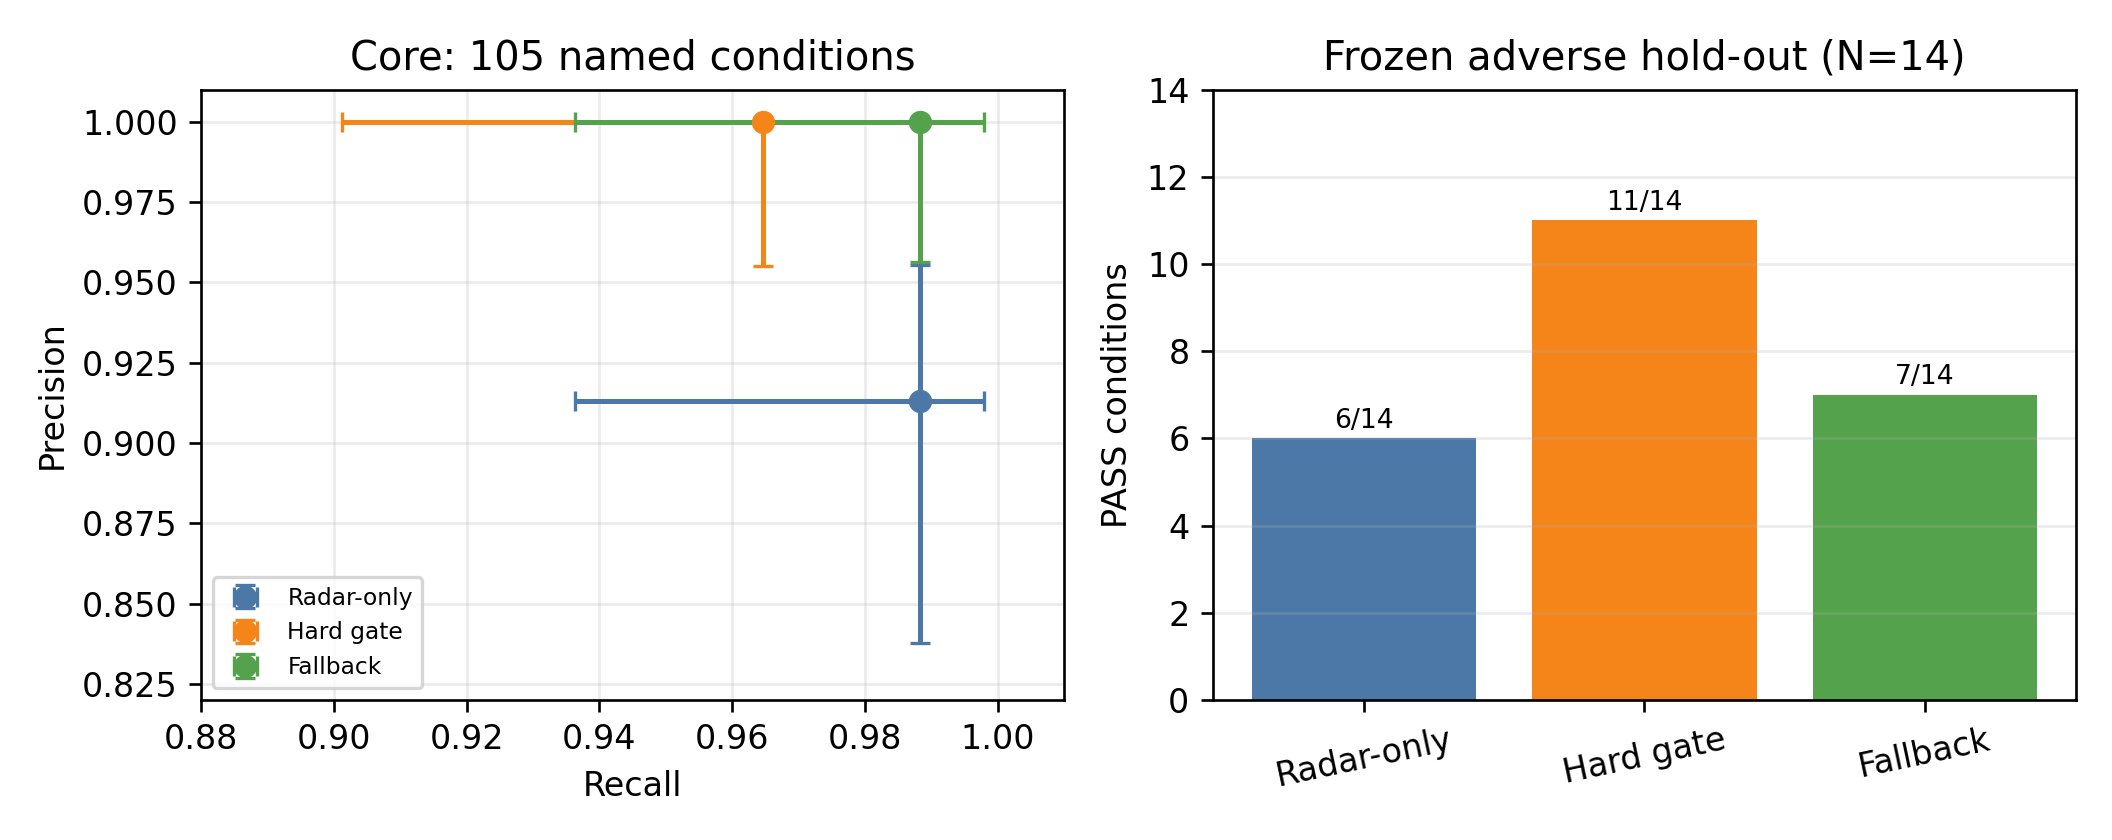
\includegraphics[width=0.90\textwidth]{scenario_level_tradeoff.png}
\caption{Frozen named-condition evidence. Left: core precision--recall and descriptive Wilson intervals. Right: system PASS on the 14-condition adverse hold-out. Neither grid estimates road prevalence.}
\label{fig:primary}
\end{figure*}

\subsection{Mechanisms at different pipeline stages}
\emph{Missing track.} The hold-out shopping cart produces at most two path
candidates and no confirmed cluster. No radar brake request reaches any gate;
a late permission override cannot recover this upstream failure. All policies
impact without braking at a median proxy speed of 49.96 km/h.

\emph{Semantic veto and late permission.} The bench forms a radar track, but no
usable car confirmation. Radar-only brakes at 12.624 m; fallback qualifies at
4.295 m; hard gating does not brake. Table~\ref{tab:severity} records pre-impact
speeds of 32.57, 54.93, and 59.95 km/h, respectively. Fallback recovers a brake
TP, not timely stopping. Relative to hard gating, radar-only lowers this proxy
by about 27.4 km/h, compared with only 5.0 km/h for fallback.

\emph{Collision despite permission.} For the traffic-warning prop, all policies
brake at 21.871 m, and camera-policy logs show confirmation rather than fallback.
All collide at 7.82 km/h. The record establishes that permission was granted;
it does not independently identify a contact-dynamics or controller defect.
It demonstrates mitigation hidden by a binary collision count.

\emph{Convincing false track.} A six-point center injection forms a confirmed
track by 0.15 s with confidence 1.0, TTC 0.89 s, and margin $-15.21$ m.
Radar-only and fallback request emergency braking; hard gating has no car
confirmation. Eight- and ten-point center/0.50-m ghosts behave similarly.
Moving the injection to 0.75 m crosses the frozen 0.65-m fallback boundary but
does not prevent radar-only braking. These are synthetic counterexamples to the
sufficiency of the emergency rule, not measurements of real ghost prevalence.

\begin{table}[t]
\caption{Hold-out severity: medians over five runs per physical condition; ghost rows aggregate 25/20 runs. Pre-impact is a last-tick proxy.}
\label{tab:severity}
\centering\scriptsize
\setlength{\tabcolsep}{3pt}
\begin{tabular}{llrr}
\toprule Mechanism & Policy & Onset / gap & Severity outcome\\ \midrule
Cart & All & no brake & 49.96 km/h pre-impact\\
Bench & Radar & 12.624 m & 32.57 km/h pre-impact\\
 & Hard & no brake & 59.95 km/h pre-impact\\
 & Fallback & 4.295 m & 54.93 km/h pre-impact\\
Warning & All & 21.871 m & 7.82 km/h pre-impact\\
\midrule
Ghost FP & Radar (25 runs) & 78.4 km/h & 3.60 s / 9.02 m/s$^2$\\
 & Fallback (20) & 78.4 km/h & 3.60 s / 9.02 m/s$^2$\\
\bottomrule
\end{tabular}
\end{table}

Every ghost false brake is a simulated stop below 1 km/h, not a one-tick pulse.
The ghost rows report onset speed, override duration, and peak deceleration;
these observations make the precision loss operationally meaningful within the
simulation. They do not quantify injury or rear-end collision risk. The shared
late cut-out FN and high-speed stopping-limit collisions are different again:
they are not evidence of a camera veto, because radar-only also fails them.

\subsection{Ablation, perturbations, and detection loss}
In the 12-condition development ablation (two repeats), full fallback passes
12/12. Hard gate and no-latch each fail two central box/barrel conditions.
Removing the path constraint adds three edge-prop false brakes; removing minimum
point count adds two weak-ghost false brakes. Removing stability/confidence or
replacing TTC-AND-margin by OR changes no outcome on this focused grid. Their
independent necessity is therefore not established. Six one-factor sensitivity
conditions show a false brake when point count is lowered and a missed central
prop when stability or TTC is tightened. No global optimum is claimed.

\begin{table}[t]
\caption{Extended outcomes by named condition, not repeated run.}
\label{tab:extended}
\centering\scriptsize
\setlength{\tabcolsep}{3pt}
\begin{tabular}{llrrrrrr}
\toprule Suite & Policy & Pass/N & TP & FP & TN & FN & Coll.\\ \midrule
Perturb. & Radar & 19/20 & 20 & 0 & 0 & 0 & 1\\
 & Hard & 15/20 & 15 & 0 & 0 & 5 & 5\\
 & Fallback & 18/20 & 20 & 0 & 0 & 0 & 1\\
\midrule
Camera off & Hard & 4/10 & 0 & 0 & 4 & 6 & 6\\
 & Fallback & 8/10 & 6 & 0 & 4 & 0 & 2\\
\bottomrule
\end{tabular}
\end{table}

Table~\ref{tab:extended} separates two perturbation failures: fallback collides
at the 19-m box gap, but avoids collision at 21 m and stops at 0.353 m, below
the 0.5-m PASS threshold. Equating every FAIL with collision would be incorrect.
With detections disabled, fallback brakes for all six positive conditions but
collides in two. Hard gate's four PASS conditions are all negatives, not
successful hazard responses. These local probes expose rule dependence, not
robustness across maps, weather, or stochastic sensor errors.

\subsection{Computation and reproducibility}
The 474 required-CUDA sessions contain 74,928 inferences and zero inference
errors. Session-median p50/p95 are 9.95/11.53 ms; the inference-weighted mean is
11.56 ms. Each fresh process has one cold start above 150 ms; the maximum is
276.10 ms. These host-measured ONNX processing times exclude radar, transport,
control, display, and actuation; they are not end-to-end ECU deadlines.

Session manifests record commit, seed, CARLA versions, model/config hashes,
configured/active providers, inference counts, and errors. Tick logs retain
track support, confidence, TTC, margin, gate reason, override, and collision.
Checkpoint keys are (scenario identifier, run index); technical recovery cannot
turn an algorithmic FAIL into a selected successful retry. Named confusion,
paired outcomes, and severity regenerate from the frozen logs without adding
or removing a run. Repository refactoring and launcher changes occurred later
and are not experimental contributions or new validation of these policies.

Source and curated evidence are indexed at
\url{https://github.com/mvhoang92/aeb}; the companion source map identifies the
frozen raw archive, derivation scripts, and checksums. Re-execution requires a
compatible CARLA installation, local model artifact, and CUDA environment.
Hashes establish artifact identity, not hardware-independent bitwise behavior.
The provenance distinction matters: regression testing of later software does
not enlarge the scientific sample or replace the archived campaign.

\section{Discussion and Validity}
\subsection{What the comparison establishes}
The results locate three different questions: did radar form a target, did the
policy permit braking, and did the permitted action achieve sufficient
mitigation? Collapsing them into one success rate obscures both the bench's late
permission and the warning prop's low-speed collision. Likewise, the emergency
rule improves core recall but admits ghosts with the same qualifying attributes.
Track persistence and point support strengthen an estimate without independently
proving a physical obstacle exists.

This is a limitation of the tested information and thresholds, not an
impossibility theorem for radar-camera fusion. Hard gating is favored by binary
hold-out PASS here, but not by bench mitigation; fallback is favored on core,
but its hold-out false brakes are full stops. We do not prescribe a universal
policy by assigning arbitrary weights to these incompatible outcomes. A useful
next comparison must include class-agnostic visual verification and a
confidence-matched soft gate before attributing gains to a new fusion algorithm.
Probabilistic methods require calibration and evidence beyond a renamed tracker
score \cite{sandblom2011threat,lindenmaier2022existence}.

The resulting answers to RQ1--RQ3 are conditional but actionable. Policy gains
can be traced to a small number of identified mechanisms rather than a generic
``fusion improvement.'' An override cannot repair the absence of an upstream
track, and passing a radar-quality threshold can both admit a ghost and delay a
real obstacle. Finally, collision avoidance, impact mitigation, and unwanted
intervention are distinct objectives. A policy that wins on one should not be
selected from a single aggregate F1 or PASS rate without specifying the intended
operating conditions and acceptable error costs. The present suite supports
these comparisons within its grid, not deployment-specific cost estimation.

\subsection{Limits of the evidence}
The experiment covers one map, ego platform, fixed seed, favorable imaging,
and an in-domain car-only detector. Repeats are correlated, and the 14-condition
hold-out was deliberately constructed with rule knowledge. It tests adverse
mechanisms rather than unbiased generalization. Point-level CARLA radar does
not reproduce full multipath physics; fault injection does not estimate real
radar-ghost frequency \cite{kraus2021ghost,magosi2022radar}. The last pre-impact
tick has 0.05-s discretization, and false-brake kinematics are not injury costs.
There is no multi-map/weather/friction sweep, real-sensor experiment, HIL,
functional-safety demonstration, or standards certification.

There is also no matched soft-gate, class-agnostic, learned, or probabilistic
baseline. The camera-veto limitation is conditional on the chosen car-only
label space, not a claim about all camera systems. Expanded baselines require a
new development/evaluation protocol; the already inspected hold-out may remain
regression data but cannot remain unseen test evidence. This restriction
preserves the present adverse results instead of tuning away the counterexamples.

\section{Conclusion}
In a fixed CARLA pipeline, emergency fallback recovers two camera-vetoed core
hazards while retaining edge-prop false-brake suppression. Four persistent
synthetic-ghost conditions reverse its advantage over hard gating on adverse
hold-out. Full-stop false brakes and delayed bench mitigation show why brake
recall and collision counts alone are insufficient. The evidence supports a
mechanism- and severity-aware comparison of permission policies, not a general
fusion advantage. Missing camera confirmation is not proof of free road, and
stable radar support is not proof of a physical hazard.

\balance
\bibliographystyle{IEEEtran}
\bibliography{references}
\end{document}
